\documentclass[answers]{exam}

%% Language and font encodings
\usepackage[english]{babel}
\usepackage[utf8x]{inputenc}
\usepackage[T1]{fontenc}
\usepackage[nomarkers,figuresonly]{endfloat}

%% Sets page size and margins
\usepackage[a4paper,margin=2cm]{geometry}

%% Useful packages
\usepackage{amsmath}
\usepackage{graphicx}
\usepackage{paralist}
\setlength\FrameSep{4pt}

\newcommand{\ptm}[1]{p_{\textsc{TM}}(#1)}
\newcommand{\plm}[1]{p_{\textsc{LM}}(#1)}
\DeclareMathOperator*{\argmax}{arg\,max}

\begin{document}
\begin{questions}
\question[10]{Experiment with stack pruning parameters. What is their affect on.'..}
\begin{framed}
\begin{compactenum}[a.]
\item log-probabilities:\\
  The log-probabilities go up with increases in $s$ and $k$, though seems to be no
  significant increase past either $s > 10$ or $k > 10$. The log-probabilities
  seem to plateau at around this point.
\item speed:\\
  The speed goes down with increases in $s$ and $k$. For $k \leq 10$ the
  decrease in speed is minimal, but for larger values of $k$, the impact of
  increasing $s$ gets bigger and bigger.
\item translations:
\item maximum log-probability:\\
  The log-probability plateaus at $-1353.247828$.
\end{compactenum}
\end{framed}


\question[15]{Define a new dynamic program for Part 2.}
\begin{framed}
  \begingroup\raggedright
  First, let us define some notation for the sum of the log-probabilities of the
  sequence $e_{1}\dots e_{k}e$ following $e'$ according to the language model: 
  \par\endgroup
  \(\!
  \begin{aligned}
    \log{\plm{e_{1}\dots e_{k}e \mid e'}}
    = \log{\plm{e_{1} \mid e'}}
    + \sum_{i=1}^{k-1}{\log{\plm{e_{i+1} \mid e_{i}}}}
    + \log{\plm{e \mid e_{k}}}
  \end{aligned}
  \)
  \\
  \begingroup\raggedright
  Secondly, we let $h(i,e) = s(0,0,i,e)$, and we define $s(k,j,i,e)$, for $k =
  j = 0 \lor k < j$, as follows:
  \par\endgroup
  \(\!
  \begin{aligned}
    &s(0,0,0,e) =
    \begin{cases}
      \epsilon         &\text{if }e = \text{START}\\
      \text{undefined} &\text{otherwise}
    \end{cases}
  \end{aligned}
  \)
  \(\!
  \begin{aligned}
    &s(0,0,i,e) = \argmax_{s(k,j,i,e')e_{1}\dots e_{n}e}
    &&\log{p(s(k,j,i',e'))} + \log{\plm{e_{1}\dots e_{n}e \mid e'}}
    \\& &&+
    \begin{cases}
      \log{\ptm{f_{i'+1}\dots f_{i} \mid e_{1}\dots e_{n}e}}
      &\text{if }k = 0 \land j = 0
      \\
      \log{\ptm{f_{k}\dots f_{j-1} \mid e_{1}\dots e_{n}e}}
      &\text{otherwise}
    \end{cases}
    \\
    &s(k,j,i,e) =
    \argmax_{s(0,0,i',e')e_{1}\dots e_{n}e}
    &&\log{p(s(0,0,i',e'))} + \log{\plm{e_{1}\dots e_{n}e \mid e'}} 
    \\& &&+\;\log{\ptm{f_{j}\dots f_{i} \mid e_{1}\dots e_{n}e}}
  \end{aligned}
  \)
  \\
  \begingroup\raggedright
  Note that $s(0,0,i,e)$ does \emph{not} denote a translation state with a hole
  in the $k^{th}$ position, as the second argument is the index of the first
  word \emph{after} the gap. It denotes a translation state without a gap.
  \par\endgroup
\end{framed}


\question[5]{What is the complexity of your Part 2 decoder? Explain your reasoning.}
\begin{framed}
\end{framed}


\question[5]{What is the mapping from hypothesis objects to stacks for Part 2?}
\begin{framed}
  Hypothesis objects are mapped to stacks as $s(k,j,i,e)\mapsto i - (k - j)$, as
  we need to subtract the number of words in the gap ($k - j$) from the number
  of words covered ($i$). Since $h(i,e) = s(0,0,i,e)$, $h(i,e)\mapsto i$ as in
  the previous model.
\end{framed}


\addtocounter{question}{1}
\question[15] Experiment with stack pruning parameters for Part 2. What is their affect on...
\begin{framed}
\begin{compactenum}[a.]
\item log-probabilities:
\item speed:
\item translations:
\item maximum log-probability:
\end{compactenum}
\end{framed}


\question[10]{Define a new dynamic program for Part 3.}
\begin{framed}
  \(\!
  \begin{aligned}
    &s(0,0,0,e) =
    \begin{cases}
      \epsilon         &\text{if }e = \text{START}\\
      \text{undefined} &\text{otherwise}
    \end{cases}
  \end{aligned}
  \)
  \\
  \(\!
  \begin{aligned}
    &s(0,0,i,e) = \argmax_{s(k,j,i,e')e_{1}\dots e_{n}e}
    &&\log{p(s(k,j,i',e'))} + \log{\plm{e_{1}\dots e_{n}e \mid e'}}
    \\& &&+
    \begin{cases}
      \log{\ptm{f_{i'+1}\dots f_{i} \mid e_{1}\dots e_{n}e}}
      &\text{if }k = 0 \land j = 0
      \\
      \log{\ptm{f_{k}\dots f_{j-1} \mid e_{1}\dots e_{n}e}}
      &\text{otherwise}
    \end{cases}
    \\
    &s(k,j,i,e) =
    \argmax_{s(k',j',i',e')e_{1}\dots e_{n}e}
    &&\log{p(s(k',j',i',e'))} + \log{\plm{e_{1}\dots e_{n}e \mid e'}} 
    \\& &&+
    \begin{cases}
      \log{\ptm{f_{j}\dots f_{i} \mid e_{1}\dots e_{n}e}}
      &\text{if }k' = 0 \land j' = 0
      \\
      \log{\ptm{f_{k}\dots f_{j-1} \mid e_{1}\dots e_{n}e}}
      &\text{if }i' = i
    \end{cases}
  \end{aligned}
  \)
\end{framed}


\question[5]{What is the computational complexity of your Part 3 decoder?}
\begin{framed}
\end{framed}


\question[5]{What is the mapping from hypothesis objects to stacks for Part 3?}
\begin{framed}
\end{framed}


\addtocounter{question}{1}
\question[5]{What is the maximum log-probability your Part 3 decoder can obtain? What do you conclude?}
\begin{framed}
\end{framed}
\end{questions}


% figures

\begin{figure}
  \centering
  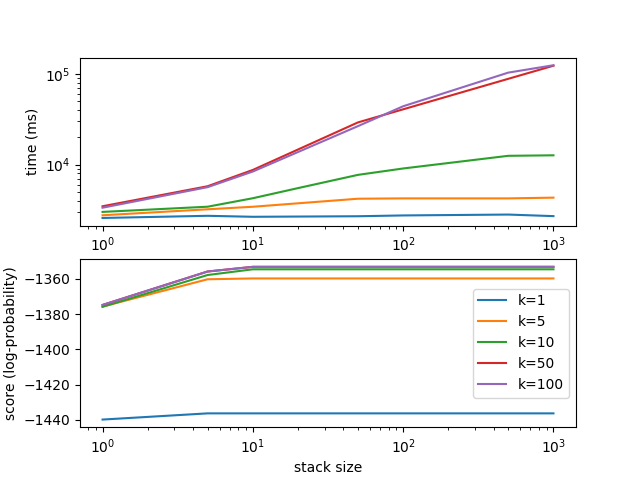
\includegraphics{fig-default}
  \caption[Experiment (baseline).]{Experiment with stack pruning parameters
    (baseline).}
  \label{fig:exp-baseline}
\end{figure}

\begin{figure}
  \centering
  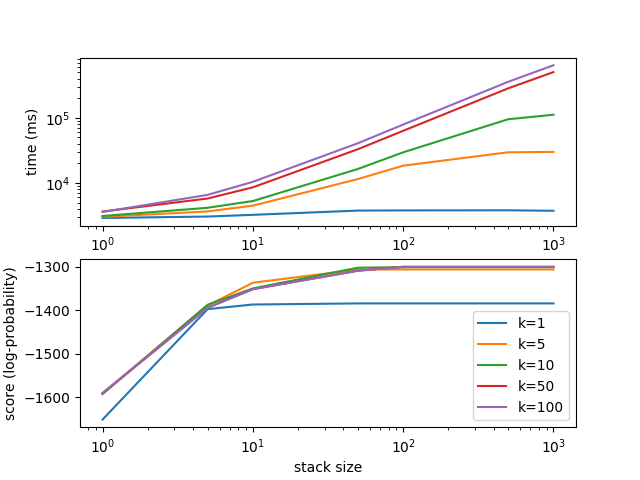
\includegraphics{fig-part2}
  \caption[Experiment (baseline).]{Experiment with stack pruning parameters
    (part2).}
  \label{fig:exp-part2}
\end{figure}

\begin{figure}
  \centering
  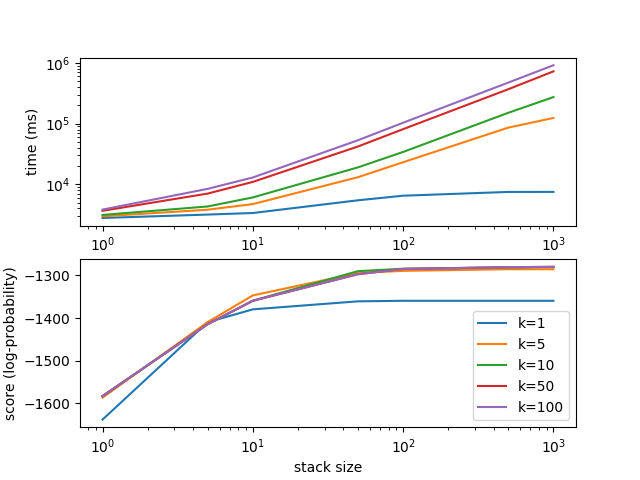
\includegraphics{fig-part3}
  \caption[Experiment (baseline).]{Experiment with stack pruning parameters
    (part3).}
  \label{fig:exp-part3}
\end{figure}


\end{document}